\section{ACP Dataset Construction}\label{sec:dataset}
% When reconstructing the phonetic system, Wang always follows the taxonomy in \textit{Qieyun} and attach pronunciations, represented by phonetic symbols, onto each initial or final category based on \textit{Qieyun} taxonomy. This reconstruction makes use of contemporaneous written materials, primarily poetic and literary materials since these works often have rigorous rhyming rule, thus similarities among certain categories, especially for syllable finals, can be deduced.
% \MY{You wanna name your dataset? i.e. AncientChinesePhones (ACP), things like this}
% \MY{Can you use 1 sentence to say why we need to combine them? like if following only 1 data, what would we miss?}
Our \textbf{ACP} (Ancient Chinese Pronunciation) dataset offers character-wise chronological data of ancient Chinese pronunciation, combining two kinds of data: the digitized \textit{Guangyun} data \cite{kanji_database_project__2004} and the phonological reconstruction result of \citet{wang_l_hanyu_2012}. For a given character, the former informs us the category it belongs to, and the latter tells us the pronunciation reconstruction results on each category.

\textit{Guangyun} is a rhyme dictionary using a special sound annotation called \textit{Fanqie}. Chinese characters are monosyllabic, i.e. all Chinese character's pronunciation correspond to one syllable, each comprised of an initial and a final\cite{duanmu2007phonology}. According to \textit{Fanqie}, each Chinese character's pronunciation is described as a combination of two representative characters, one for its \textit{initial} and another for its \textit{final} as shown in Figure \ref{fig:fanqie}. 
    \begin{figure}[ht]
        \centering
        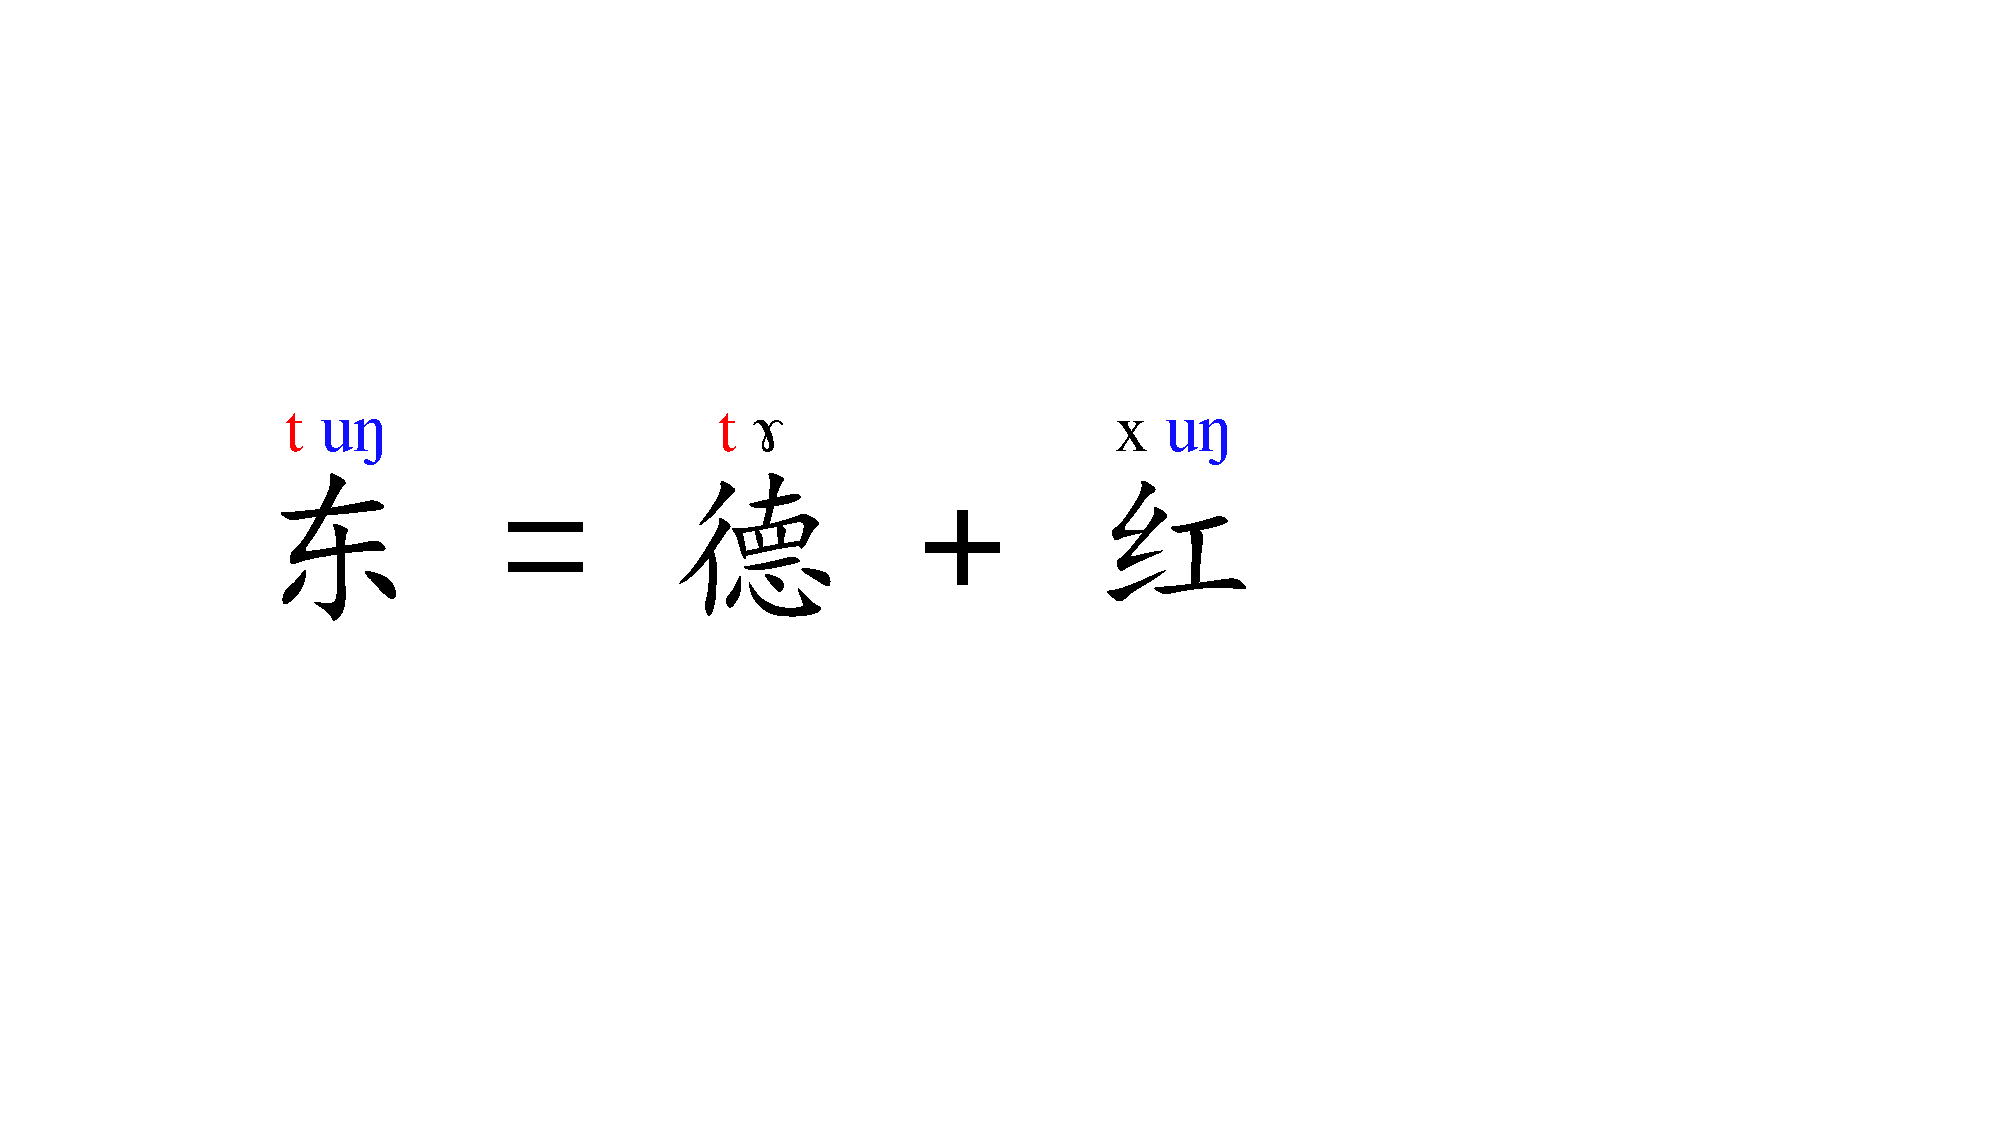
\includegraphics[width=5cm]{images/fanqie.pdf}
        \caption{Method of \textit{Fanqie}:  \begin{CJK*}{UTF8}{gbsn}“东”\end{CJK*} belongs to category \begin{CJK*}{UTF8}{gbsn}“德”\end{CJK*}(\textipa{[t]}) for initial and to category \begin{CJK*}{UTF8}{gbsn}“红”\end{CJK*}(\textipa{[uN]})for final.}
        \label{fig:fanqie}
    \end{figure}

Under this taxonomy, there are 38 categories of initials and 298 categories of finals. The aim of phonological reconstruction is to attach the exact pronunciation (denoted by IPA phoneme) onto each initial and final category for targeted period. These information can be found in \citet{wang_l_hanyu_2012}'s reconstruction results of Chinese phonology, which includes the evolution of Chinese pronunciation system from PreQin (-206 BC) to modern Chinese (AD 1912-) at 9 different representative time points. We have only selected results for 6 historical periods after that MiddleTang dynasty: \texttt{MiddleTang, LateTang, Song, Yuan, MingQing and Modern}, represented by the midpoint in time of each historical period (AD 709, AD 898, AD 1120, AD 1324, AD 1640, AD 1968), since these reconstruction results are more consistent among different linguists\cite{zuofan_1936,wang_l_hanyu_2012}. See Figure \ref{fig:timeline} for the Chinese history timeline.
% \MY{so T is for MiddleTang? These abbreviations are a bit weird, consider using ABCDE instead, as they can suggest an order. Or you can list the current abbreviations in brackets in lines 152-155 as i just did} 

When constructing ancient Chinese pronunciation for each character in ACP dataset, 4 possible cases are presented (More examples in  \appref{app:reconstruction}):

    \paragraph{Direct determination of pronunciation} 
    If the exact pronunciation is directly given for one category, then the given IPA phoneme is attached onto each character within this category. For example, \begin{CJK*}{UTF8}{gbsn}“波”\end{CJK*} belongs to initial category of \begin{CJK*}{UTF8}{gbsn}“帮”\end{CJK*} and [p] is attached to category \begin{CJK*}{UTF8}{gbsn}“帮”\end{CJK*}, then the initial IPA of \begin{CJK*}{UTF8}{gbsn}“波”\end{CJK*} is [p].
    This is the case for pronunciation system of MiddleTang since all characters strictly belongs to its category denoted in \textit{Guangyun}.

    \paragraph{Rule-based determination of pronunciation}
    If there exists several possible pronunciations for the same category,
    then the linguistic rules given by Wang are applied to help choose the correct one. Rules on initials' pronunciation are usually based on finals' category, and rules on finals' pronunciation are usually based on the articulation information recorded in \textit{Guangyun}
    \footnote{The articulation information is only vaguely recorded in \textit{Guangyun}.}. For example, \begin{CJK*}{UTF8}{gbsn}“砩”=“帮”+“废”\end{CJK*} and \begin{CJK*}{UTF8}{gbsn}“碑”=“帮”+“支”\end{CJK*} both belongs to initial category of \begin{CJK*}{UTF8}{gbsn}“帮”\end{CJK*}, but given the linguistic rule that \begin{CJK*}{UTF8}{gbsn}“帮”\end{CJK*} represents [f] only under the case when fianl category is \begin{CJK*}{UTF8}{gbsn}废\end{CJK*}, and represent [p] in other cases, we attach [f] as \begin{CJK*}{UTF8}{gbsn}砩\end{CJK*}'s initial IPA and [p] as \begin{CJK*}{UTF8}{gbsn}碑\end{CJK*}'s initial IPA.
    This is the case for LateTang and Song period since a small amount of categories' pronunciation has encountered rule-based change.
    
    \paragraph{Arbitrary determination of pronunciation}
    
    If a category-wise pronunciation reconstruction is no given due to the complexity of the language system's evolution, then we manually digitize Wang's example on several representative characters' pronunciation. This is the case for Yuan and MingQing
    % \MY{use full spelling for these dynasties in main text}
    pronunciation system since the overall categorization has significantly changed compared to MiddleTang phonology system.
    
    \paragraph{Converted pronunciation}
    For modern Chinese language system, we take Mandarin as its representative. Since Mandarin is a living language, we directly convert the pronunciation to IPA representation.

\begin{figure*}[ht]
    \centering
    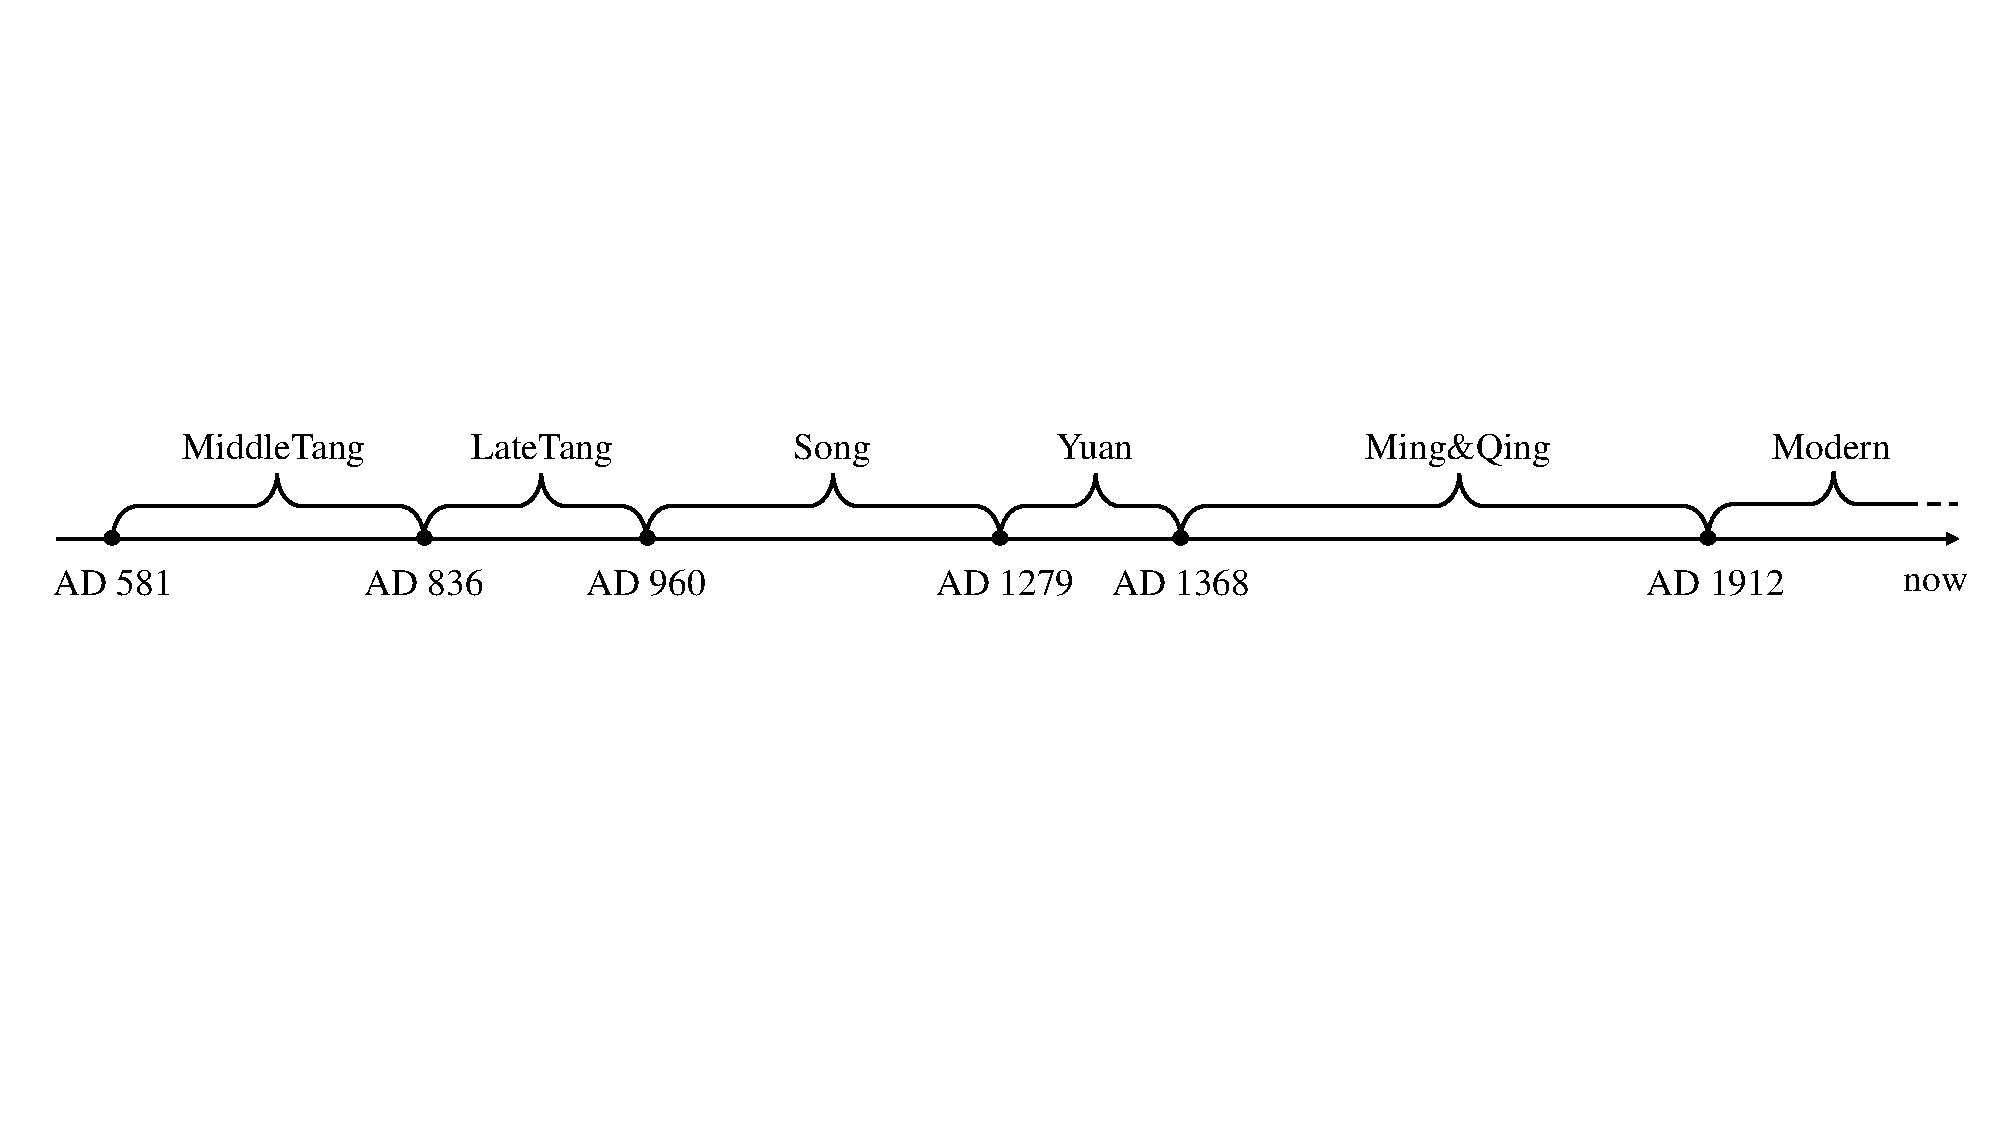
\includegraphics[width=0.9\textwidth]{images/history_tl.pdf}
    \caption{China history timeline. The 6 pronunciation systems represents the overall spoken language form in a certain period of time. 
    % \KZ{abbreviation to one letter. delete dynastie name, match result with model figure
    % Fig still very blurry when magnified. The Sui, Tang etc. below the time axis is not needed when you have the red part on the top. A dynasty should be a time period and not a point anyway. Also Republic Period should be ROC, and PRC is 1949 not 1945.}
    }
    \label{fig:timeline}
\end{figure*}

Following these IPA symbols and conditions, we manually attach the initials and finals, take all the available records as single entries and left the unknown entries blank. Meanwhile, another articulation information, the tone, is much more complicated to trace since rhyme dictionaries focus on initials' and finals' taxonomy and only give vague description on tone\cite{wang_l_hanyu_2012}. The linguistic reconstructions have no consistent results \cite{zhiping_1986_tone, xiangdong_earlytang, wuyun_1982}, thus neither encoded into ACP dataset for any of the time period. 
% \MY{need ref and a bit explanation on why tone information is difficult to trace}

According to the articulation feature, we further divide the final part into Medial, Nucleus and Coda as shown in \figref{fig:split}. The medial is an optional part of the final, usually has short and soft sounding, connecting initial and final. The nucleus is the main and non-empty vowel in final. The coda is attached to nucleus which can only be consonant or empty. Finally, each single entry in our dataset is composed of 4 parts: Initial-I, Medial-M, Nucleus-N and Coda-C, either empty (denoted by ``-") or non-empty (denoted by one IPA phoneme). Example of complete and incomplete sets of pronunciations for one character in the dataset can be found in \tabref{tab: Dataset example}. The final dataset contains 17,001 entries for each of the 17,001 Chinese characters in MiddleTang, LateTang, Song and Modern historical period\tabref{tab:dataset}. Meanwhile, only 1,402 entries for Yuan and 1,519 entries for MingQing is provided while other filled with [UNK] due to the inherent incompleteness in linguistics reconstruction.

\begin{table}[ht]
    \centering
    \footnotesize
    \begin{tabular}{l@{\hskip 4pt}c@{\hskip 4pt}c@{\hskip 4pt}c@{\hskip 4pt}c@{\hskip 4pt}c@{\hskip 4pt}c}
    \hline
     & \textbf{T} & \textbf{L} & \textbf{S} & \textbf{Y} & \textbf{Q} & \textbf{M}\\
    \hline
    \textbf{Entries} & 17,001 & 17,001 & 17,001 & 1,420 & 1,519 & 17,001\\
    \textbf{Coverage} & 100\% & 100\% & 100\% & 8.25\% & 8.93\% & 100\%\\
    \hline
    \end{tabular}
    \caption{The statistics of ACP dataset. Abbreviations: T - MiddleTang, L - LateTang, S - Song, Y - Yuan, Q - MingQing, M - Modern.}
    \label{tab:dataset}
\end{table}

\begin{figure}[h!]
    \centering
    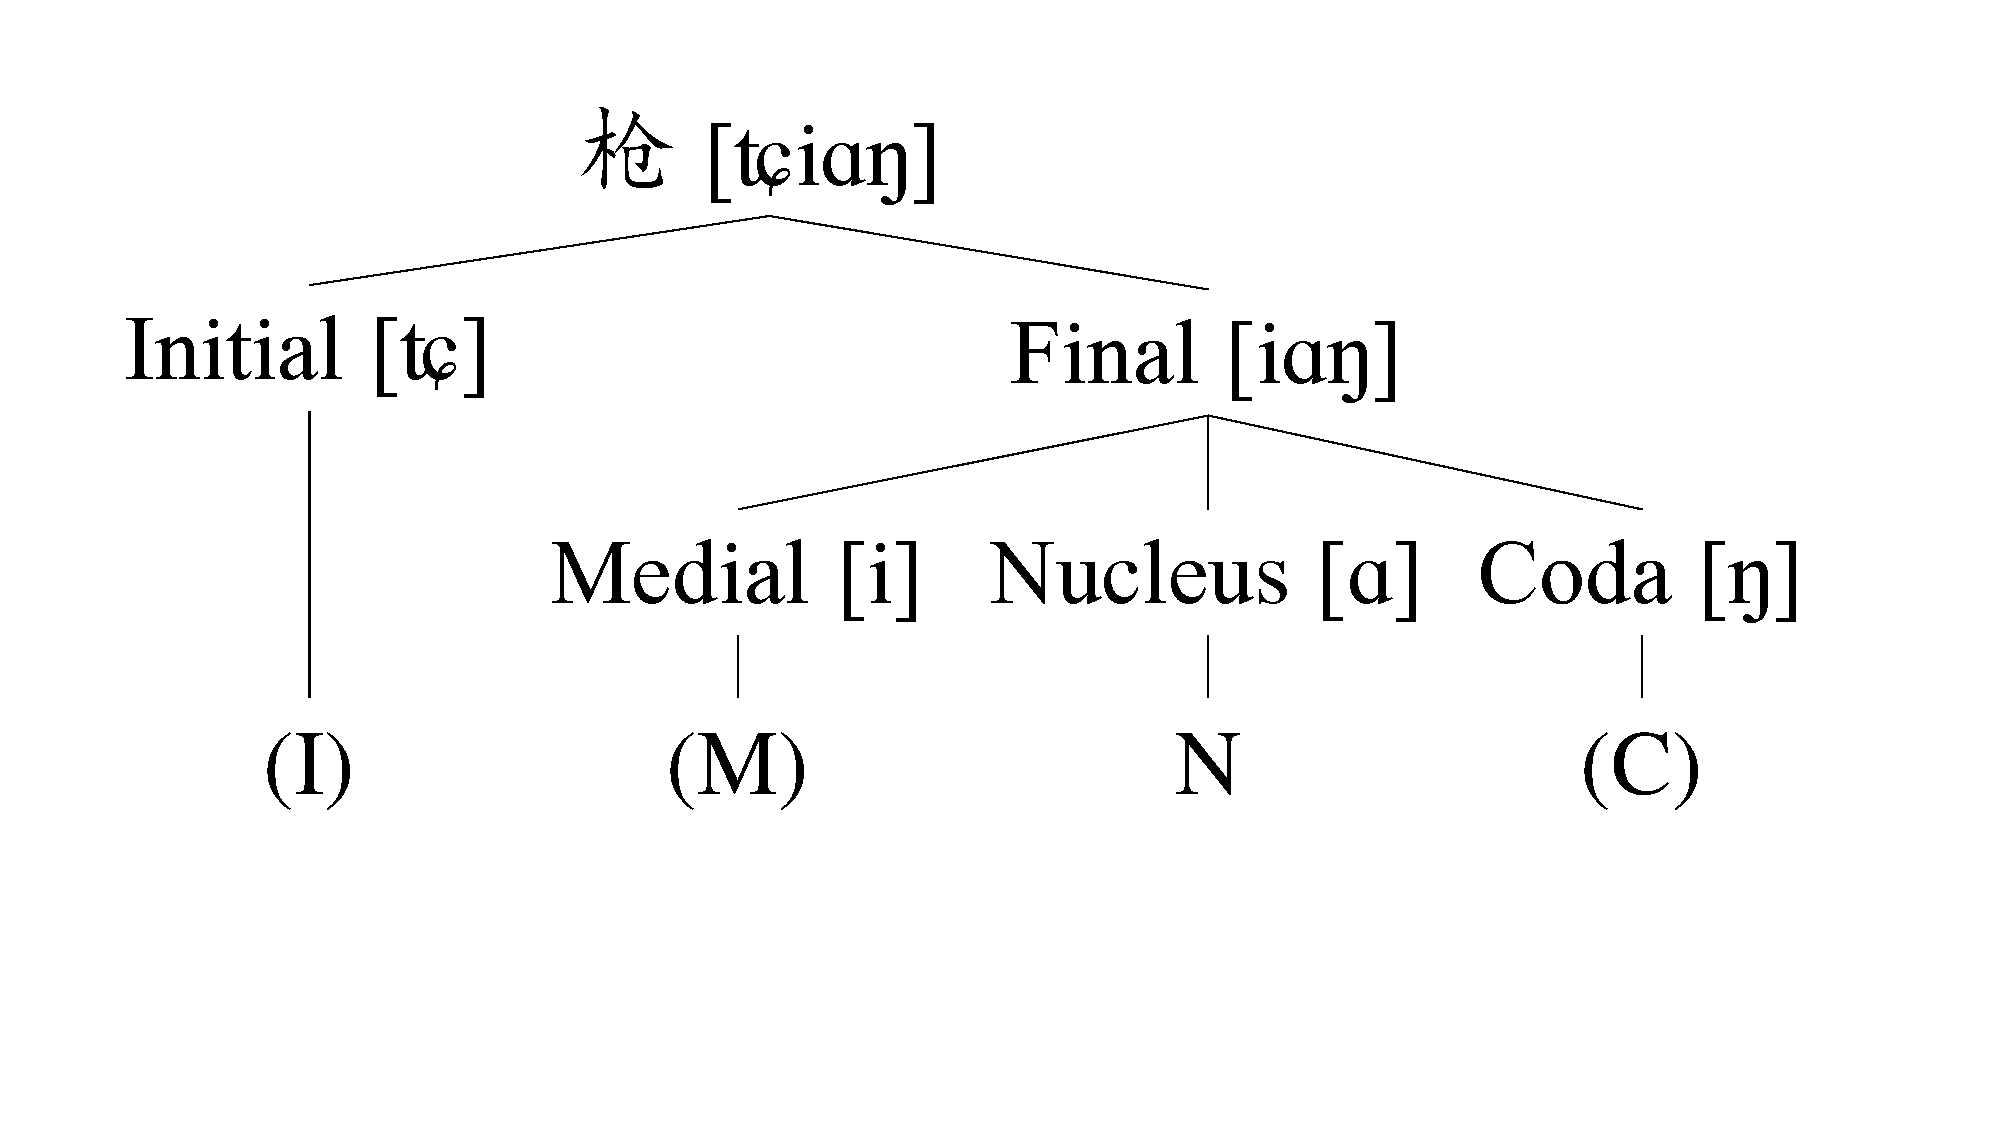
\includegraphics[width=7cm]{images/split.pdf}
    \caption{The phoneme sequence is split into initial, medial, nucleus and coda, where initial, medial and coda are optional.
    }
    \label{fig:split}
\end{figure}


\begin{table*}[ht]
    \centering
    \footnotesize
    \resizebox{\linewidth}{!}{
    \begin{tabular}{ccccccccccccccccccccccccc}
    \hline
\multicolumn{1}{c}{\multirow{2}{*}{Character}} &
  \multicolumn{4}{c}{\textbf{MiddleTang}} &
  \multicolumn{4}{c}{\textbf{LateTang}} &
  \multicolumn{4}{c}{\textbf{Song}} &
  \multicolumn{4}{c}{\textbf{Yuan}} &
  \multicolumn{4}{c}{\textbf{MingQing}} &
  \multicolumn{4}{c}{\textbf{Modern}} \\
\multicolumn{1}{c}{}&I&M&N&C& I & M & N  & C & I & M & N  & C & I & M & N  & C & I  & M & N  & C & I  & M & N  & C \\
    \hline
\begin{CJK*}{UTF8}{gbsn}纣\end{CJK*} & d & i & ou & - & \textctd & i & \textipa{@u} & - & t\textctc & i & \textipa{@u} & - & t\textctc & i & \textipa{@u} & - & \textrtails & - & \textipa{@u} & - & t\textrtails  & - & ou & - \\
\begin{CJK*}{UTF8}{gbsn}雍\end{CJK*} & \textipa{\textglotstop} & i & u & \textipa{N} & \textipa{\textglotstop} & i & u & \textipa{N} & j & i & u & \textipa{N} & \multicolumn{4}{c}{UNK} & j & - & y & \textipa{N}  & j & - & u & \textipa{N} \\
\begin{CJK*}{UTF8}{gbsn}皙\end{CJK*} & s & - & i & k & s & i & \textipa{@} & k & s & - & i & t & \multicolumn{4}{c}{UNK} & \multicolumn{4}{c}{UNK} & \textctc & - & i & - \\
    \hline
    \end{tabular}}
    \caption{Example of complete and incomplete sets in the dataset.}
    \label{tab: Dataset example}
\end{table*}

% \MY{From my perspective, our main contribution is the digital version of this ancient chinese pronunciation dataset. Hence, we'd better give a screenshot/smaller version of the dataset to showcase what you did here, including the timeline, different characters, their respective initial, nucleus and coda. Also, a link to full access of Yvonne's excel (the dataset itself, but in a visualized version and a csv/json file) is preferred. I think Yvonne maybe you can take some time to do this?}\YV{dataset example-OK. Online access of dataset-We can directly put it in the same github repository.}
